% document
\documentclass[10pt,graphics,aspectratio=169,table]{beamer}
\usepackage{listings}
\usepackage{csquotes}
\usepackage{hyperref}
% theme
\usetheme{metropolis}
% packages
\title{Lesson 1}
\author{Christian Schwarz, Jakob Krebs}

\begin{document}
\maketitle

\begin{frame}{Contents}
	\tableofcontents
\end{frame}

\section{Introduction}
\begin{frame}{Getting started}
  \begin{itemize}
  \item we will use mostly linux
  \item all slides and examples will be available on github
    \url{https://github.com/jkrbs/c_lessons}
  \item all tasks can be send to us via e-mail and we will prvide feedback
    \url{c-lessons@deutschland.gmbh}
  \item information on our course will be available on \url{https://users.ifsr.de/~krebs/c-lessons}
  \item weekly lessons \textbf{Mondays, 13:00-14:30}
  \end{itemize}
\end{frame}

\begin{frame}{development envirement}
  \begin{itemize}
  \item you can use any editor of your choice
  \item you also can use an ide like vscode, atom, \ldots
  \item we will use a commandline, vim and gcc
  \end{itemize}
  \alert{\textbf{DO NOT USE AN IDE TO GET STARTED!}}
\end{frame}


\begin{frame}[fragile]{gcc for Unix-based operating systems}
	Ubuntu / Debian:
	\begin{lstlisting}[numbers=none]
$ sudo apt-get install gcc
\end{lstlisting}
	\bigskip
	Arch Linux:
	\begin{lstlisting}[numbers=none]
$ sudo pacman -S gcc
\end{lstlisting}
	\bigskip
	Mac OS X:
	\begin{lstlisting}[numbers=none]
$ brew install gcc
\end{lstlisting}
	\bigskip
	... and you're done ;-)
\end{frame}

\begin{frame}{gcc for Windows 10 (using \textit{bash})}
	For convenience you should use the new Ubuntu-based Linux subsystem.\\
	\bigskip
	\begin{itemize}
		\item In \textit{Settings}, got to \textit{Update \& Security} $>$ \textit{For Developers}
			and switch to \textit{Developer Mode}
		\item In the \textit{Control panel}, go to \textit{Programs} $>$ \textit{Turn Windows Features On or Off}
			and enable the \textit{Windows Subsystem for Linux (Beta)}
		\item Reboot as you're prompted
		\item Search for ``bash'' and run the \textit{bash} command
		\item Follow the installation instructions
	\end{itemize}
	\bigskip
	You may now continue as if you were using Ubuntu ;-)
\end{frame}

\begin{frame}[fragile]{gcc for older versions of Windows (using \textbf{cygwin})}
	We highly recommend using the \href{https://chocolatey.org/}{Chocolatey} package manager.\\
	\begin{itemize}
		\item Follow the link and the instructions on the website to install it
	\end{itemize}
	\bigskip
	Install cygwin (launch the shell as an administrator!):
	\begin{lstlisting}[numbers=none]
$ choco install cygwin
$ choco install cyg-get
\end{lstlisting}
	\bigskip
	Install gcc and optionally vim: {\scriptsize(\href{https://github.com/chocolatey/chocolatey-coreteampackages/issues/176#issuecomment-212939458}{How to fix the "Cannot find file" error})}
	\begin{lstlisting}[numbers=none]
$ cyg-get gcc-core vim
\end{lstlisting}
	\bigskip
	Now start \textit{cygwin} to get a command line similar to Unix.
\end{frame}

\section{Hello World!}
\subsection{}
\begin{frame}[fragile]{The first program}
	\begin{itemize}
		\item Create a new file named ``\textbf{main.c}''.
		\item Open it in your text editor of choice.
		\item Fill it as follows:
	\end{itemize}
	\begin{lstlisting}
#include <stdio.h>

int main(void) {
	printf("Hello World!\n");
	/* Print "Hello World!" on the
	   command line */
	return 0;
}
\end{lstlisting}
\end{frame}
\begin{frame}[fragile]{From source to binary}
    \begin{figure}
        \centering
        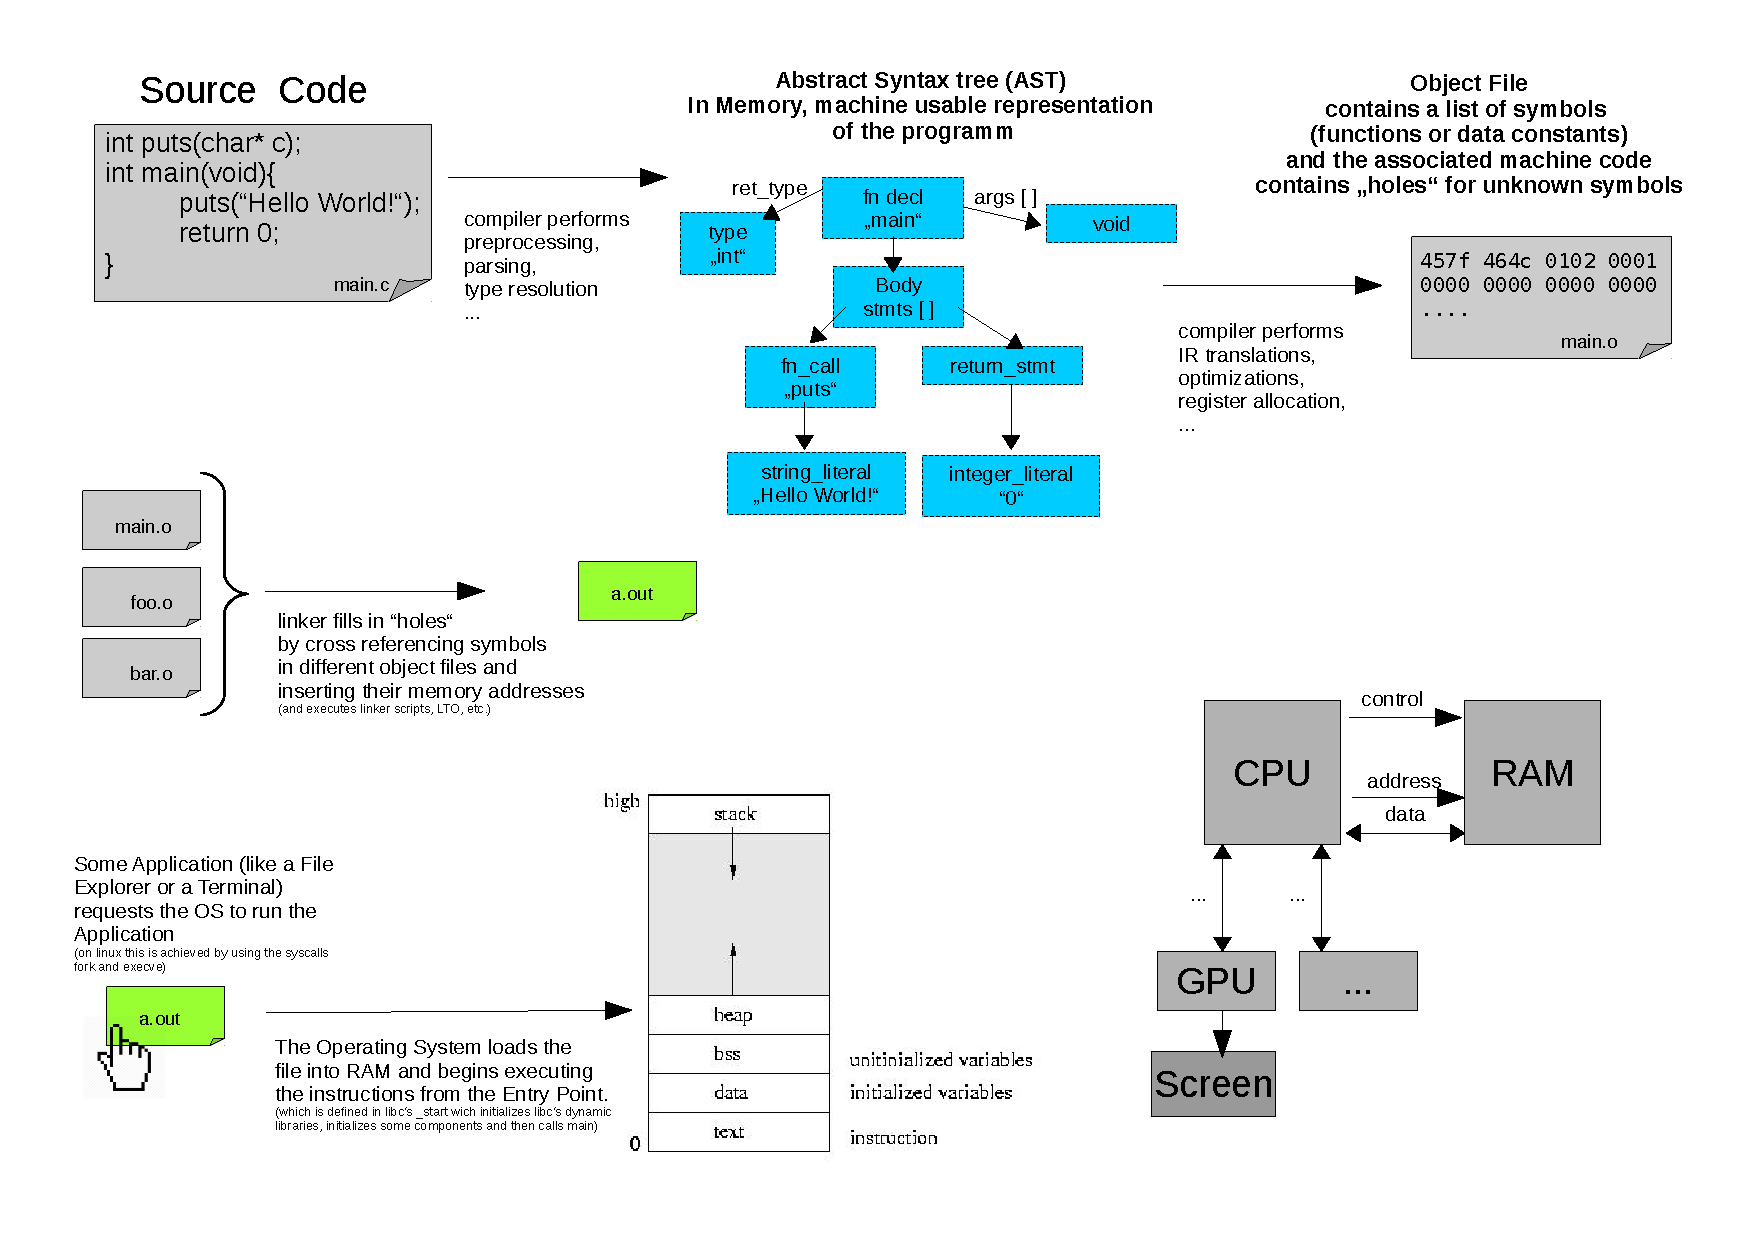
\includegraphics[width=0.6\linewidth]{img/FromSourceToBin.pdf}
    \end{figure}
\end{frame}
\begin{frame}[fragile]{Compiletime vs Runtime}
    \begin{figure}
        \centering
        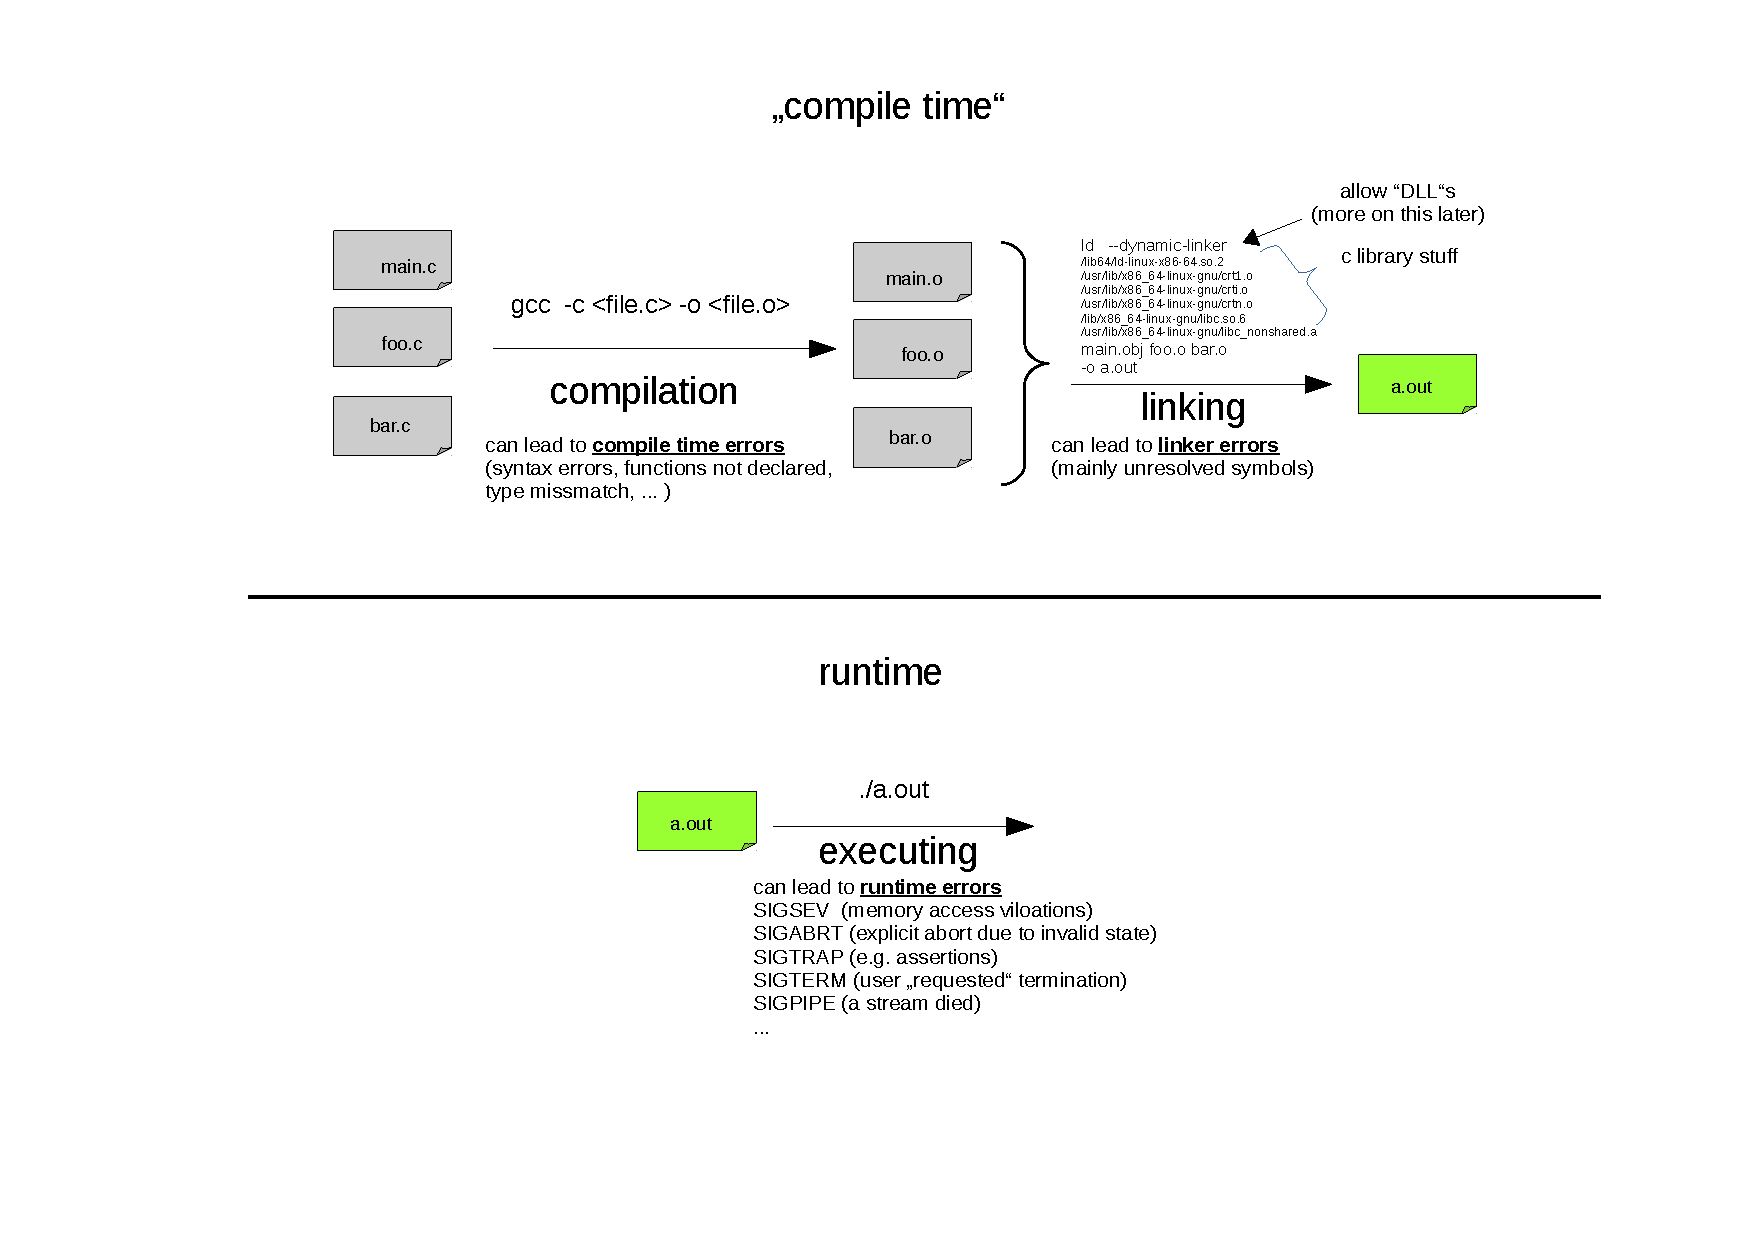
\includegraphics[width=0.9\linewidth]{img/ComptimeRuntime.pdf}
    \end{figure}
\end{frame}
\section{Program structure}
\subsection{}
\begin{frame}[fragile]{A basic program}
	\begin{columns}[T]
		\column{.6\textwidth}
		\begin{lstlisting}
#include <stdio.h>

int main(void) {

	printf("Hello World!\n");
	/* Print "Hello World!" on the
	   command line */

	return 0;
}
\end{lstlisting}
		\column{.4\textwidth}
		
		\ \\$\left. \begin{array}{c}\\\end{array}\right\rbrace $ Preprocessor statements
		\ \\\ \\$\left. \begin{array}{c}\\\\\\\\\\\\\end{array}\right\rbrace $ Main function
	\end{columns}
\end{frame}
\begin{frame}[fragile]{Preprocessor statements}
	\begin{itemize}
		\item Processed before compilation
		\item Have their own language; start with a \textit{\#}
	\end{itemize}
	\begin{lstlisting}
#include <stdio.h>
\end{lstlisting}
	\begin{itemize}
		\item Includes the \textit{input/output header} from the \textbf{C standard library}
		\item Needed to use \textit{printf()}
	\end{itemize}\ \\ \ \\
	Preprocessor statements have way more use cases,\\
	but they form their own language which is very different from actual C.\\
	\bigskip
	In this course, we will use them for inclusions only.
\end{frame}
\begin{frame}[fragile]{The main function}
	\begin{itemize}
		\item Core function of every program
		\item Exists \textbf{exactly once} in every program
		\item Called on program start
	\end{itemize}
	\begin{lstlisting}
int main(void) {
\end{lstlisting}
	\begin{itemize}
		\item As a function, \textit{main()} can take parameters and return a value
		\item Get used to \textit{void} and \textit{int}. They will be explained later
		\item '$\lbrace$' marks the start of the main function scope
	\end{itemize}
\end{frame}
\begin{frame}[fragile]{The main function scope}
	\begin{itemize}
		\item Contains program statements
		\item They are processed from top to bottom
	\end{itemize} \ \\
	\ \\
	\begin{lstlisting}
	return 0;
}
\end{lstlisting}
	\begin{itemize}
		\item Last statement; ends main function (and thus the whole program)
		\item \textit{0} tells the OS that everything went right
		\item '$\rbrace$' marks the end of the main function scope
	\end{itemize}
\end{frame}
\begin{frame}[fragile]{Statements}
	\begin{itemize}
		\item Instructions for the computer
		\item End with a \textit{;} (semicolon)
	\end{itemize}
	\begin{lstlisting}
	printf("Hello World!\n");
\end{lstlisting} \ \\ \ \\
	\begin{itemize}
		\item Here is the empty statement:
	\end{itemize}
	\begin{lstlisting}[numbers=none]
	;
\end{lstlisting}
	\begin{itemize}
		\item All statements are located in function blocks
	\end{itemize}
\end{frame}
\begin{frame}[fragile]{Comments}
	\begin{itemize}
		\item Information for you and others who use your code
		\item Cut out before compilation
	\end{itemize}
	Single-line comments:
	\begin{lstlisting}
	// Prints "Hello World!" on the command line
\end{lstlisting}
	Block comments (multi-line):
	\begin{lstlisting}
	/* Prints "Hello World!"
	   on the command line */
\end{lstlisting}
	Better style of block comments:
	\begin{lstlisting}
	/*
	 * Prints "Hello World!"
	 * on the command line
	 */
\end{lstlisting}
\end{frame}
\section{Style}
\subsection{}
\begin{frame}[fragile]{A few words on style}
	\begin{itemize}
		\item There can be multiple statements on one line
		\item Indentation is not necessary at all
		\item<2-> \textbf{But}...
	\end{itemize}
	\ \\
	\begin{uncoverenv}<2->
	\begin{lstlisting}
#include <stdio.h>
int
main	(        void ){printf("Hello World!\n");
		// Prints
/*"Hello World!"			*/
		return 0;}
\end{lstlisting}
	\end{uncoverenv}
\end{frame}
\begin{frame}[fragile]{Write enjoyable code}
	\begin{itemize}
		\item Put each statement onto its own line
		\item Indent every statement in the main function by one \textit{tab}\\
		 or a fixed number of \textit{spaces}
		\item Decide on a commenting style and stick to it\\
		(\textit{/* .. */} recommended)
		\item Leave blank lines between different parts of the program
		\item Use \textit{spaces} and \textit{newlines} consistently
	\end{itemize}
	\begin{lstlisting}[showspaces=true,showtabs=true]
int main(void) {
	printf("Hello World!");
	/* Prints "Hello World!" */
	return 0;
}
\end{lstlisting}
\end{frame}


% nothing to do from here on

\end{document}
